\startchapter{Theory}
\label{chapter:theory}

\newlength{\savedunitlength}
\setlength{\unitlength}{2em}

The \textbf{Standard Model of Particle Physics (SM)} is a quantized relativistic field theory that describes all known elementary particles, as well as their interactions via three of the four known fundamental forces. It has been tested extremely rigorously since its development in the 1960s and 1970s, and in every case its predictions have held true. The final piece of the puzzle fell into place with the experimental verification of the existence of the Higgs Boson in 2012. (cite https://www.sciencedirect.com/science/article/pii/S037026931200857X).

Despite its success, however, the SM is considered an incomplete theory. It does not describe the interaction of matter via the fourth fundamental force, gravity, nor does it account for the existence of \textit{dark matter} in our universe, or the asymmetry between the observed amounts matter and anti-matter. These shortcomings provide motivation to extend the SM by searching beyond it for new phenomena.

This chapter will provide a short overview of the SM theory, before describing some of the deficiencies that motivate extending it.

\section{The Standard Model}

\subsection{The Particles}
The elementary particles of the Standard Model are shown in Figure \ref{fig:standardmodel}. They can be categorized into two groups: \textit{fermions} and \textit{bosons}. \textit{Fermions} carry half-integer spin, and constitute the matter that surrounds us. For each fermion there also exists a corresponding anti-particle with an opposite electric charge. In this document anti-particles will be denoted either by the charge (e.g. $e$ vs. $e^{-}$) or by a bar overhead e.g. ($t$ vs. $\bar{t}$). The fermions can be further divided into two groups: \textit{leptons} and \textit{quarks}. \textit{Leptons}, the most familiar of which is the electron, interact via the weak force and, if electrically charged, the electromagnetic force. They come in three flavour generations, each of which has a neutral particle (\textit{neutrino}) and a charged fermion with charge -1. Unlike leptons, which regularly exist freely, \textit{quarks} exist mostly in bound states called \textit{hardrons}, the most well-know of which are the proton and neutron composed of ($u,u,d$) and ($u,d,d$) quarks respectively. Like leptons, quarks come in three generations, each of which has a pair of particles with electric charges +2/3 and -1/3. They interact via all three forces of the standard model: strong, weak, and electromagnetic.

\begin{figure}[h]
    \centering
    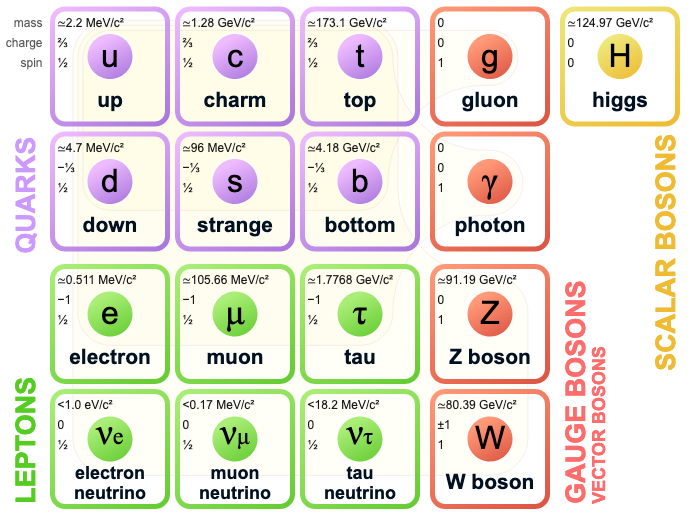
\includegraphics[width=0.8\textwidth]{Figures/1/sm.png}
    \caption{The elementary particles of the Standard Model}
    \label{fig:standardmodel}
\end{figure}

\textit{Bosons} carry integer spin, and mediate the forces via which particles interact. Massless \textit{gluons} and \textit{photons} as well as massive W and Z bosons are spin-1 vector bosons, while the Higgs Boson is a spin-0 scalar boson. The massive W and Z vector bosons are the carriers of the weak force, the photon carries the electromagnetic force, and the gluons carry the strong force binding quarks. Along with interacting with fermions via exchange, bosons are also able to interact among themselves. $W$ bosons are able to directly interact with both $Z$ bosons and and photons, as well as self-interacting. Gluons can also self-interact, but $Z$ bosons and photons cannot. The Higgs boson interacts with all massive particles, including self-interaction, and it is via their interaction with the Higgs field that massive bosons obtain their mass.

\subsection{Quantum Electrodynamics (QED)}
\textit{Quantum Electrodynamics} (QED) is a quantum field theory of electrodynamics and the electromagnetic force. It describes the interaction of electrically charged particles via the exchange of photons. Mathematically, QED is an abelian (commutative) gauge theory with the gauge group $U(1)$. The fundamental interactions of the theory are: the emission or absorption of a single photon by a charged particle and the creation or annihilation of a pair of charged particles. These interactions can all be represented by various orientations of the Feynman vertex shown in Figure ~. 
\begin{figure}[h!]
    \centering
    \feynmandiagram [horizontal=a to b] {
    % i1 -- [fermion] a -- [fermion] i2,
    a[particle=\(\gamma\)] -- [photon] b,
    f1[particle=\(\bar{f}\)] -- [fermion] b -- [fermion] f2[particle=\(f\)],
    };
    \caption{The fundamental QED vertex.}
    \label{fig:QEDvertex}
\end{figure}

\subsection{Weak Interactions}
The weak force, in contrast to the electromagnetic force, is mediated by the exchange of massive vector bosons $W^+$, $W^-$, and $Z$. Owing to the charge of the W bosons, and the fact in contrast to the electromagnetic force neutral fermions also interact via the weak force, there are many more possible fundamental interactions. Figure ~ shows the vertices corresponding three such interactions: Fermions interacting with the $Z$ boson in a similar vertex to that of Figure ~ shown in (a), a charged lepton and neutrino interacting with a $W$ boson shown in (b), and a quark-antiquark pair interacting with a $W$ boson shown in (c).

\begin{figure}[h!]
    \begin{subfigure}{.5\textwidth}
        \centering
        \feynmandiagram [horizontal=a to b] {
        a[particle=\(Z\)] -- [photon] b,
        f1[particle=\(\bar{f}\)] -- [fermion] b -- [fermion] f2[particle=\(f\)],
        };
        \caption{Z interaction.}
        \label{fig:EWvertexa}
    \end{subfigure}
    \begin{subfigure}{.5\textwidth}
        \centering
        \feynmandiagram [horizontal=a to b] {
        a[particle=\(W^{\pm}\)] -- [photon] b,
        f1[particle=\(\nu\)] -- [fermion] b -- [fermion] f2[particle=\(l\)],
        };
        \caption{W interaction with leptons.}
        \label{fig:EWVertexb}
    \end{subfigure}
    \newline
    % \centering
    \begin{subfigure}{1\textwidth}
        \centering
        \feynmandiagram [horizontal=a to b] {
        a[particle=\(W^{\pm}\)] -- [photon] b,
        f1[particle=\(\bar{q}\)] -- [fermion] b -- [fermion] f2[particle=\(q\)],
        };
        \caption{W interaction with quarks.}
        \label{fig:EWVertexc}
    \end{subfigure}
    \caption{Some fundamental weak interaction vertices.}
    \label{fig:EWVertices}
\end{figure}

At high energy scales, the aforementioned electromagnetic force and the weak force unify to become the electroweak interaction. Glashow, Salam, and Weinberg's theory unites to two forces into a single $U(1) \otimes SU(2)$ gauge theory. 

\subsection{Quantum Chromodynamics (QCD)}
\textit{Quantum Chromodynamics} (QCD) is the theory describing the strong interaction between gluons and quarks. It is again a gauge theory, this time with the SU(3) symmetry group. There are three colour charges associated with this group, which are carried by both quarks and gluons. Each of the 8 gluons carries a unique colour charge and anti colour charge pair, while quarks carry a single colour charge. Because they carry colour charge, gluons are able to both interact with quarks and self-interact. This gives rise to several possible interaction vertices in the theory, some of which are shown in Figure ~.

\begin{figure}[H]
    \begin{subfigure}{.5\textwidth}
        \centering
        \feynmandiagram [horizontal=a to b] {
        a[particle=\(g\)] -- [gluon] b,
        f1[particle=\(\bar{q}\)] -- [fermion] b -- [fermion] f2[particle=\(q\)],
        };
        \caption{Gluon interaction with quarks.}
        \label{fig:QCDvertexa}
    \end{subfigure}
    \begin{subfigure}{.5\textwidth}
        \centering
        \feynmandiagram [horizontal=a to b] {
        a[particle=\(g\)] -- [gluon] b,
        f1[particle=\(g\)] -- [gluon] b -- [gluon] f2[particle=\(g\)],
        };
        \caption{Gluon self-interaction.}
        \label{fig:QCDVertexb}
    \end{subfigure}
    \caption{Some fundamental QCD interaction vertices.}
    \label{fig:QCDVertices}
\end{figure}

\subsection{The Higgs Boson}
Electroweak theory alone does not contain a mechanism to provide particles with mass. This contrasts with the observed reality that all fermions as well as $W$ and $Z$ bosons are in fact massive. If the lagrangian of these theories were to contain mass terms, they would lose their gauge invariance and the standard model would not be renormalizable. Instead, these particles acquire their mass through the \textit{Higgs Mechanism}.

A new Higgs Field $\Phi$ is introduced, with a Lagrangian which can be written as:
$$ L_{Higgs} = (D_{\mu}\Phi)^{\dagger}D^{\mu}\Phi + V(\Phi) $$
Where $D_{\mu}$ is the gauge covariant derivative of the electroweak theory. In order for the Lagrangian to remain gauge invariant the Higgs potential $V(\Phi)$ must take the form:
$$V(\Phi) = {\mu}^2{\Phi} + {\lambda}{\Phi}^4 $$
where $\lambda$ and $\Phi$ are free parameters. $\lambda$ is forced to be greater than 0 by requiring that the potential have a stable minimum. This leads the potential to have two different possible shapes, shown in Figure ~, given the sign of $\mu^2$

\begin{enumerate}
    \item ${\mu^2 > 0}$: The trivial case of a parabolic potential with a minimum at $\Phi = 0$ arises.
    \item ${\mu^2 > 0}$: A potential with a minimum at:
     $$|\Phi| = v = \sqrt{\frac{\mu^2}{\lambda}}$$ 
     arises, where $v$ is known as the vacuum expectation value. This minimum is occupied by infinitely degenerate states. This is the case that gives rise to the Higgs mechanism.
\end{enumerate}

In the second case, the ground states occupying the minimum are not equivalent under gauge transformation, which breaks the Electroweak gauge symmetry. The masses of particles are then determined by the strength of their coupling to the Higgs field.

\section{Beyond the Standard Model}
The Standard Model as described above has proven extremely robust through precise experimental testing. There are, however, many remaining questions in physics that cannot be answered within its confines. Some of those not further explored in this thesis include: whether or not there is a quantum theory of gravity that can tie it to the SM, the exact value of the neutrino masses and whether they are Majorana particles (their own antiparticles), and what the cause is of the matter-antimatter asymmetry in the universe. The fact that these questions are unanswered in the standard model tells us we must search deeper, and test beyond its limits.

\subsection{Dark Matter}
Another currently open question is the nature of dark matter. Astrophysical observations including the dynamics of galaxy clusters (cite Zwick) and rotational curves of galaxies (cite https://ui.adsabs.harvard.edu/abs/1980ApJ...238..471R/abstract) are not explained under Einstein's theory of gravitation by visible matter alone. Several theories have arisen over time to explain this discrepancy, including that Einstein's theory is not correct at galactic scales, or that these galaxies contain ordinary matter that is somehow unobservable to us. 

Most evidence, however, points to the existence of a new type of matter that interacts gravitationally but not electromagnetically with ordinary matter. Perhaps the most clear evidence for this theory comes from observations of the bullet cluster (cite https://arxiv.org/pdf/astro-ph/0608407.pdf), a pair of colliding clusters of galaxies. In such a scenario, with some normal matter and some dark matter in each cluster, the matter would collide and interact, slowing it down, while the dark matter would pass through largely undisturbed. In the case of the bullet cluster, this separation is observed when comparing the distribution of mass in the galaxies measured by gravitational lensing and the distribution of normal matter in the form of galaxy plasma, measured as emitted x-ray radiation. Figure ~ shows the observed separation, with gravitational density in blue and x-ray density in pink.

\subsection{Dark Higgs Boson Model}
This work involves a search for dark matter produced in association with a new hypothetical scalar "dark Higgs" boson $s$ *Add footnote - s is not strange quark*. In this model the dark matter particle $\chi$ is a majorana fermion, who's mass is generated by a Higgs mechanism in the dark sector. This also generates the new $s$ particle. If the mass of $s$ is less than that of $\chi$ then the relic density is set by the process $\chi\chi \rightarrow ss$, followed by the decay of $s$ to standard model partices. The addition of a further paricle, such as a massive $Z'$ boson allows this model to be probed at a collider.

The model proposes that the dark matter particle $\chi$ obtains its mass from the vacuum expectation value (vev) $w$ of a new Higgs field $S$. A new $U(1)'$ gauge group is proposed, uder which $S$ carries a charge $q_s$. As a result, the vev $w$ of $S$ breaks the gauge symmetry, and through this mechanism the mass of the corresponding $Z'$ boson is generated. Additionally, the dark matter particle $\chi$ couples to the $Z'$ boson, allowing all particles in the new dark sector to interact. This gives rise to the renormalizable interaction Lagrangian, which can be written in terms of four independent parameters $m_{\chi}$, $m_{Z'}$, $m_{s}$, and $g_{\chi}$:

$$ L_{\chi} = -\frac{1}{2}g_{\chi}Z'^{\mu}\bar{\chi}\gamma^5\gamma_{\mu}\chi - g_{\chi}\frac{m_{\chi}}{m_{Z'}}s\bar{\chi}\chi + 2g_{\chi}Z'^{\mu}Z'_{\mu}(g_{\chi}s^2 + m_{Z'}s) $$

where $m_{\chi}$ is the mass of the dark matter particles, $m_{Z'}$ is the mass of the $Z'$ boson, $m_{s}$ is the mass of the dark higgs, and $g_{\chi}$ is the dark matter coupling constant.

Additionally, the coupling of the $Z'$ boson to standard model quarks is described by the Lagrangian:

$$ L = -g_qZ'^{\mu}\bar{q}\gamma_{\mu}q $$

where $g_q$ is the coupling constant between $Z'$ and quarks.

A final free parameter $\theta$ is the non-zero mixing angle between the SM Higgs boson and the dark Higgs boson. The dark Higgs obtains its couplings to standard model particles through this mixing, and therefore shares the same standard model decay branching fractions as the SM Higgs boson.

For the analysis described in this work the free parameters are set as:

\begin{itemize}
    \item $g_{\chi} = 1$
    \item $m_{\chi} = 200 GeV$
    \item $m_{Z'}$ allowed to vary
    \item $m_s$ allowed to vary
    \item $g_q = 0.25$
    \item $\theta = 0.01$ 
\end{itemize}

The values of $g_{\chi}$ and $g_{q}$ were chosen to facilitate comparison with other LHC searches with similar models, which traditionally use the values selected. The value of $\theta$ was chosen to match that of (Cite DH paper). Its precise value is not relevant to this search, but it is sufficiently large that the dark Higgs decays promptly to standard model states. The varied values $m_s$ and $m_{Z'}$ form the parameter space covered by this search. 
